\documentclass{sig-alternate-05-2015}

\usepackage{float}

\begin{document}


	
% Copyright
\setcopyright{acmcopyright}
%\setcopyright{acmlicensed}
%\setcopyright{rightsretained}
%\setcopyright{usgov}
%\setcopyright{usgovmixed}
%\setcopyright{cagov}
%\setcopyright{cagovmixed}


% DOI
\doi{10.475/123_4}

% ISBN
\isbn{123-4567-24-567/08/06}

\title{Experiment on Performance Difference between Test Driven Development and Code First Test After}

\numberofauthors{3}
\author{
% 1st. author
\alignauthor
	Mads Riisom\\
	\affaddr{University of Southern Denmark}\\
	\affaddr{Odense, Denmark}\\
	\email{marii13@student.sdu.dk}
% 2nd. author
\alignauthor
	Tenna Cortz\\
	\affaddr{University of Southern Denmark}\\
	\affaddr{Slagelse, Denmark}\\
	\email{tecor13@student.sdu.dk}
% 3rd. author
\alignauthor
	Henrik Bolding Frank\
	\affaddr{University of Southern Denmark}\\
	\affaddr{Odense, Denmark}\\
\email{hefra13@student.sdu.dk}
}

\maketitle
\begin{abstract}
\textit{Background:} Test Driven Development (TDD) is considered a good approach concerning productivity compared to the more common Code First Test After (CFTA) approach, and it works by implementing the tests first, when the tests are done the developer implements just enough logic to pass the test. \textit{Goal:} The group aim to investigate if there is a performance gain in using TDD over CFTA. \textit{Method:} The group performed an experiment using 65 test subjects, who received one of four coding tasks, the tasks had the same end result, but the tasks were described and had to be solved using different approaches with either step by step instructions (Sliced) or free text (Non-sliced) requirement descriptions. Further the subjects had to answer a questionnaire before and after the coding task. \textit{Result:} The experiment showed that with this test group the approach was less important than how detailed the task was described.

\textit{Conclusion:} From this experiment the group cannot make any generalized conclusion as the test group is not a representative of the target group, but there seem to be no real difference between TDD and CFTA.

\end{abstract}

\section{Experiment Explanation}
The experiment aimed to investigate the performance difference between TDD and the more common CFTA approach, with either step by step instructions (Sliced) or free text (Non-sliced). To investigate this the group performed an experiment using third semester Software Engineering bachelor students at SDU as test subjects.


Before and after the experiment the students were handed a questionnaire; the first with questions regarding their perception of their own skill level, and the latter with questions about how well they thought they had performed during the experiment.


The experiment was split into 4 different tasks:
\begin{itemize}
	\item Non-sliced, test-last (NSTL)
	\item Sliced, test last (SLTL)
	\item Non-sliced test first (NSTF)
	\item Sliced, test first (SLTF)
\end{itemize}

These tasks were randomly distributed among the students with no knowledge to the group of which students got which specific task.


At the beginning of the experiment the students received a code skeleton to work from, to ensure that the assignments would have a similar structure, and therefore it would be easier to compare the results. The code completeness and correctness was then evaluated using an ordinal scale, from where it were decided whether the student were in one of the following three states; failed, critical and passed. The code and questionnaires were then analysed to see if there was a correlation between testing before or testing after writing the code, and the task description's granularity.


While performing the experiment the group participated in a supporting capacity, as well as observers and coordinators. While helping the students with the difficult parts of the experiment, the group gained more insights into the different tasks, and the students approaches to the tasks. These insights could influence the group's objectivity to the experiment process as well as their perception of the results.

\section{Descriptive Statistics}
The dataset the experiment is based on, consists of 65 data points, from where 3 data points were rejected as they did not fulfill the requirements for the questionnaires, in other words they were either double or incomplete submission. Therefore, only 62 data points are represented in the following section.

All the subjects had submitted a zip-file containing their solution based on the code skeleton provided for the experiment. The 3 states the submissions were categorized in, were evaluated as if it was a real exam submission.
The states were divided as follows:

\begin{itemize}
	\item 23 - failed attempts, where the solution had no chance to fulfill the requirements.
	\item 16 - critical state attempts, where the probability for the submission is high, but the fulfillment of the requirements is questionable.
	\item 23 - passed attempts, where the solutions were fulfilling the requirements.
\end{itemize}

\begin{figure}[H]
	\centering
	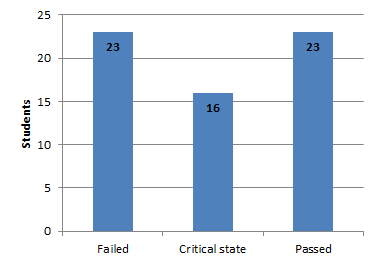
\includegraphics[width=0.4\textwidth]{img01}
	\caption{Distribution of student's performance}
\end{figure}

Figure 1 represents the distribution of student's performance in the experiment, where the evaluation of their submitted code were divided into the three states.\\

As the distribution of the tasks were random, and each student got exactly one task. The number of students receiving the individual tasks were distributed as illustrated in figure 2:

\begin{figure}[H]
	\centering
	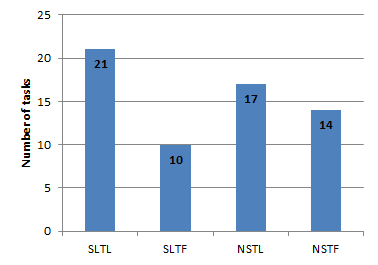
\includegraphics[width=0.4\textwidth]{img02}
	\caption{Task distributions}
\end{figure}

38 students were to do the experiment with the test-last approach, where 24 students had to do the test-first approach. Further it is an exceptionally case that both the sliced and non-sliced tasks were equally distributed with 31 of each.

After the assessment of the student submitted code, it is possible to look at the answers of the questionnaires. Shown in figure 3 the student's perception of their own programming experience in these fields; General programming, C{\#}, Visual Studio, Unit testing, NUnit testing framework and Test-driven development (TDD).
The students were rating their experience on the scale: None, Novice, Intermediate and Expert.

\begin{figure}[H]
	\centering
	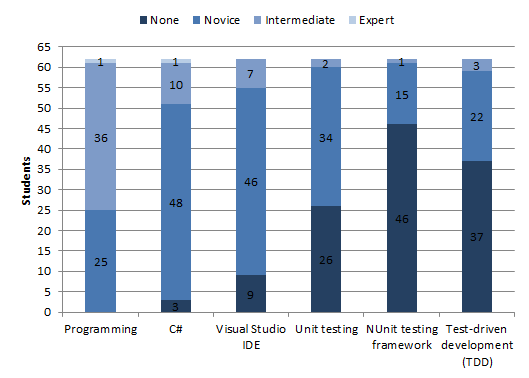
\includegraphics[width=0.4\textwidth]{img03}
	\caption{Student's own experience rating}
\end{figure}

It is important to see how the subject's self perception of their experience in TTD also seems to be based on which task the subject were handed.

\begin{figure}[H]
	\centering
	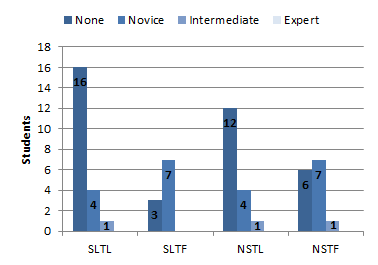
\includegraphics[width=0.4\textwidth]{img04}
	\caption{TDD experience in tasks}
\end{figure}

When looking at figure 3 and 4, there are more people with none TDD-experience in the test-last approach, which also is an exceptionally case.

The experiment aimed to investigate the performance difference between Test-Driven Development (TDD) and the more common Code First Test After (CFTA) approach, with either step by step instructions (Sliced) or free text (Non-sliced).\\

As the experiment aimed to investigate the performance based on the four tasks distributed among the students, figure 5 shows the code states divided by the tasks.

\begin{figure}[H]
	\centering
	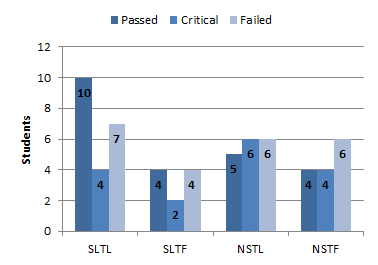
\includegraphics[width=0.4\textwidth]{img05}
	\caption{Student's task performance}
\end{figure}

As it is stated in figure 5, there are a tendency for the students' submissions to pass with sliced tasks.

\section{Findings}

Figure 6 shows the distributions between the students self-rating of programming experience level (None, Novice, Intermediate, Expert), and their correlating submission state (Passed, Critical, Failed), divided into each of the tasks respectively.
It is important to notice that there were no students who have rated their programming experience  as "None" which means that the group could have excluded this in figure 6-9. These are however included in the diagrams as it was an option in the pre-questionnaire, and therefore if excluded, would give a skewed view of the students programming experience levels. This does also apply for the "Expert" ratings which will be described below.

\begin{figure}[H]
	\centering
	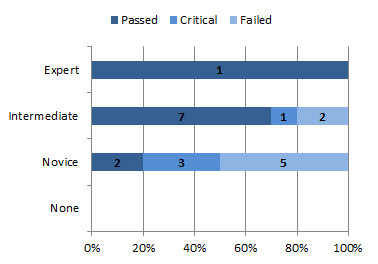
\includegraphics[width=0.4\textwidth]{img06}
	\caption{SLTL percentage distributions with relative task numbers}
\end{figure}

Here it is seen that 100\% of all students who rated their programming experience to be "Expert" has submitted a solution that fulfilled the requirements satisfying, where it was only 70\% and 20\% in respectively "Intermediate" and "Novice".
It is important to notice that there were only one student who rated him- or herself as an "Expert" in programming experience, which means that he could have been excluded from the statistical analysis of this task, as the "Expert" percentage are misleading the reader. The rest of the percentages are for the critical submissions 10\% and 30\%, and for the failed submissions 20\% and 50\% respectively for the "Intermediate" and the "Novice" students.

\begin{figure}[H]
	\centering
	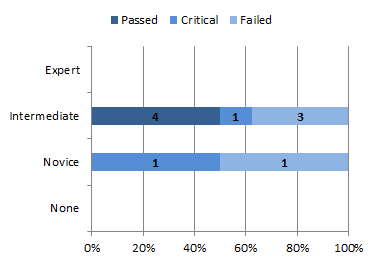
\includegraphics[width=0.4\textwidth]{img07}
	\caption{SLTF percentage distributions with relative task numbers}
\end{figure}

In figure 7 it is seen that only 50\% of the "Intermediate" students submitted solutions which fulfilled the requirements satisfying, where there are none "Novice" students who did. On the other hand it is seen that it is respectively 12.5\% and 50\% in the "Intermediate" and "Novice" who were in the Critical state. The last percentages is 37.5\% and 50\% for respectively the "Intermediate" and the "Novice" students.

\begin{figure}[H]
	\centering
	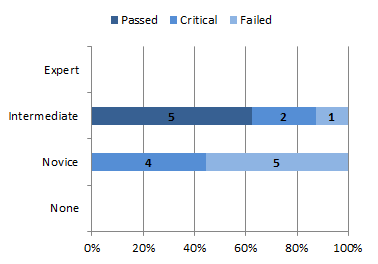
\includegraphics[width=0.4\textwidth]{img08}
	\caption{NSTL percentage distributions with relative task numbers}
\end{figure}

Figure 8 shows the distribution of the students' experience and states of the NSTL tasks. Here it is also seen that it is only the students who have rated themselves as "Intermediate" experienced in programming, who submitted solutions that fulfilled the requirements with 62.5\%. This means that the "Novice" students had a distribution, with 44.5\% critical and 55.5\% failed submissions. Whereas the "Intermediate" students had 25\% critical and 12.5\% failed solution submissions.

\begin{figure}[H]
	\centering
	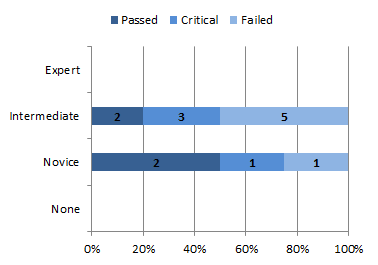
\includegraphics[width=0.4\textwidth]{img09}
	\caption{NSTF percentage distributions with relative task numbers}
\end{figure}

Figure 9 shows the distribution of the student's experience and states of the NSTF tasks. Here it is seen that both the "Intermediate" and the "Novice" students have submitted solutions that fulfilled the requirements, with a distribution of 20\% and 50\% respectively. Further the critical is distributed 30\% and 25\% where the failed is distributed 50\% and 25\% respectively for the "Intermediate" and the "Novice" students.

Figure 10 is a visualization of the total normalized data divided into the four different tasks. These data is calculated based on the weights: Passed=1, critical=0.5, failed=0.01.

\begin{figure}[H]
	\centering
	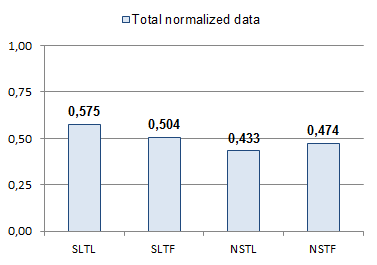
\includegraphics[width=0.4\textwidth]{img10}
	\caption{Total normalized data distributed in tasks}
\end{figure}

It is seen that the students who had the sliced tasks performed better than the students who had the non-sliced tasks.

Figure 11 shows "Novice" and "Intermediate" normalized data respectively, in accordance to the total normalized data.

\begin{figure}[H]
	\centering
	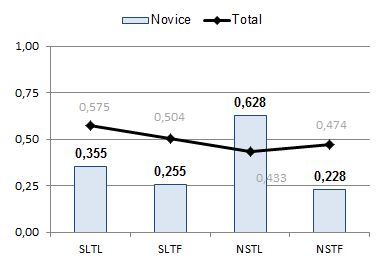
\includegraphics[width=0.4\textwidth]{img11}
	\caption{Novice normalized data distributed in tasks in accordance to total normalized data}
\end{figure}

In figure 11 it is illustrated that the "Novice" normalized data is lower than the total in all tasks but in the NSTL task. This data suggest that people who rate their programming experience as "Novice" is more predisposed to doing well when given the NSTL task, than when given one of the other tasks.

\begin{figure}[H]
	\centering
	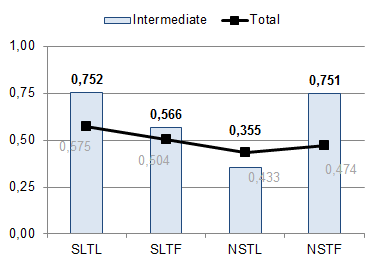
\includegraphics[width=0.4\textwidth]{img12}
	\caption{Intermediate normalized data ditsributed in tasks in accordance to total normalized data}
\end{figure}

Figure 12 shows that the "Intermediate" normalized data is higher than the total in all tasks but in the NSTL. Which suggest that people who rates their programming experience at "Intermediate" is more predisposed to do worse when given the NSTL tasks in comparison if given one of the other tasks.

\section{Threats to validity}

The threats to the Internal validity of this experiment are mostly related to the selection process. The experiment was conducted while the students were performing a test, which would indicate that they were highly motivated to perform well.\\

Further External threats to the validity were amongst others the \textit{Interaction of setting and treatment}, as the test subjects were given small simple tasks to complete, which does not represent a real world setting the results from an experiment in the field might vary. \textit{Interaction of history and treatment} is an important factor as the subjects had received lectures in all the topics tested in the experiment a few weeks up to the experiment. The participants were not representative of the target group (Software Developers) which also had an effect on the results, as they were unable to perform at the same level as the level as the target group.\\

One of the major Social threats were the subjects inability to work alone, as some talked together during the experiment, which was not intended. The group did not consider \textit{Hypothesis guessing} a threat for the coding part of the experiment, but had to reevaluate it after the end of the experiment, as the subjects did not have more than 5  weeks of experience with TDD from received lectures. This might have impacted the subjects answers more or less in favor of TDD in the pre and post questionnaires. Another threat to the Social validity comes from the human discomfort from being evaluated, which can have influenced the results.\\

The principal Conclusion validity is affected by the \textit{heterogeneity of the subjects} was rather large, as the test subjects was still only in the start of their university education, so their previously programming ability still played a major role in their programming proficiency which is also concerning the External validity. The conclusion validity is generally strong because of the high \textit{Statistical Power} in having a large group of participants, but the group do not claim that the results can be generalized for the entire software developer population. 

\section{Discussion}

When the group have conducted the experiment, it was clear that there were some aspects that could have been improved, or done differently. First of all the group had different roles during the experiment, as they both acted as supporters and observers for the experiment. The supporting role was expressed during the experiment, when the students had any questions regarding the experiment in general and when more specific problems appeared, when eg. their IDE did not work properly. Whereas the observation-role were at any other point, to keep track of how the students performed the experiment. These roles could have been divided so some members of the group only acted like supporters and others as observators, which could have giving the group a different point of view as well as both having the subjective and objective view on the experiment process.\\

The subjective view gave the group the knowledge that it seemed like the students did not actually read the experiment task properly, where the objective view gave the group knowledge that the students did talk together even though they specifically had been told not to.

The coding submissions were a direct result of the students programming level in general and their TTD experience was not as high as the group expected, based on their answers in the pre- and post questionnaires. Further the different tasks gives an idea that the sliced tasks were easier for the students to do than the non-sliced tasks, as the passed-level in these are lower than the critical and failure-levels.

\section{Conclusion And Future Work}
In this study the group performed an experiment to investigate if there was an increase in productivity when the using TDD instead of CFTA. The test subjects were not representative of the target group of software developers so these findings only reflect how TDD and CFTA compare when used by students. 

But the experiment indicates that for students considering themselves as Novices making the tests first yielded worse results then Test Last. The students considering themselves as intermediate the Test first seemed to yield the best results. But these results has to be tested further to make any generalized conclusion as there is no clear trend in the results.

In the future the group would like to perform a similar test on a group which has a closer relation to the actual target group. The group would also investigate if it would be possible to use a metric to determine a subject's programming proficiency objectively instead of using the user's opinion. This will hopefully lead to a more general conclusion regarding the performance differences regarding TDD and CFTA.

\begin{thebibliography}{3}

\bibitem{fucci1}
  D. Fucci, B. Turhan, M. Oivo,
  \emph{On The Effects of Programming and Testing Skills on External Quality and Productivity in a Test-Driven Development Context},
  Oulu, Finland.
  
\bibitem{fucci2}
  D. Fucci, B. Turhan,
  \emph{A Replicated Experiment on the Effectiveness of Test-first Development},
  Oulu, Finland,
  2013.
  
\bibitem{fucci3}
  D. Fucci, B. Turhan, M. Oivo,
  \emph{Impact of Process Conformance on the Effects of Test-driven Development},
  Oulu, Finland,
  2014.

\end{thebibliography}

\section{Acknowledgments}

First of all, the group wants to thank Dr. Marco Kuhrmann for his participation and help in this experiment. Especially for providing the necessary communication with the former of the experiment kit, and the provided tools and data.\\

The group also wants to thank Davide Fucci, Burak Turhan, Markku Oivo from University of Oulu for providing the experiment kit used in this experiment.\\

Thanks to all students of 3. semester Software Engineering 2016 of University of Southern Denmark for participating in this project.

\end{document}
